\documentclass{article}
\usepackage{graphicx} % Required for inserting images
\usepackage{enumitem}
\usepackage{xcolor}
\usepackage{listings}

\setlength{\oddsidemargin}{-0.25in}
\setlength{\topmargin}{-0.5in}
\setlength{\headheight}{0cm}
\setlength{\headsep}{0cm}
\setlength{\textheight}{10in}
\setlength{\textwidth}{7in}
\setlength{\topskip}{0cm}

\begin{document}

\noindent\textbf{ComS 472 - PS4 \quad Due: Oct 6, 2024 \quad Name: Aren Ashlock}

\begin{enumerate}

% ------------------------------------- 1 DONE -------------------------------------

\item \textbf{(23 pts)} (Exercise 5.8) Consider the two-player game with its starting position shown in the figure below. Player $A$ moves first. The two players take turns moving, and each player must move his token to an open adjacent space in either direction. If the opponent occupies an adjacent space, then a player may jump over the opponent to the next open space if any. (For example, if $A$ is on 3 and $B$ is on 2, then $A$ may move back to 1.) The game ends when one player reaches the opposite end of the board. If player $A$ reaches space 4 first, then the value of the game to $A$ is +1; if player $B$ reaches space 1 first, then the value of the game to $A$ is $-1$.

\begin{center}
    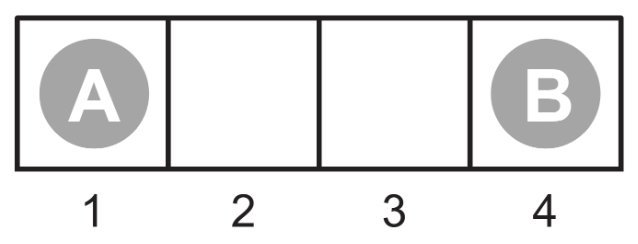
\includegraphics[scale=0.5]{472-PS4-Q1.png}
\end{center}

    \begin{enumerate}[label=($\alph*$)]
    
    % ----------------------------------- 1a DONE -----------------------------------
    
    \item \textbf{(7 pts)} Draw the complete game tree, using the following conventions:

    \begin{itemize}
        \item Write each state as ($s_A$,$s_B$), where $s_A$ and $s_B$ denote the token locations.
        \item Put each terminal state in a square box and write its game value in circle.
        \item Put \textit{loop states} (states that already appear on the path to the root) in double square boxes. Since their value is unclear, annotate each with a “?” in a circle.
    \end{itemize}

    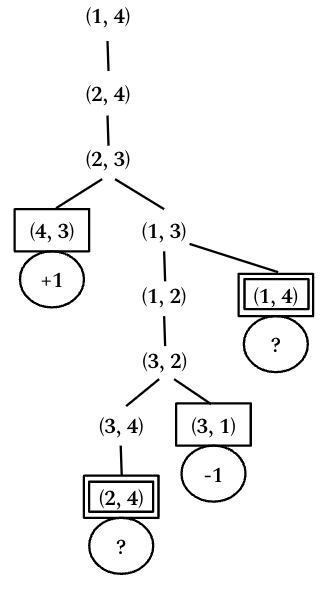
\includegraphics[scale=0.5]{472-PS4-Q1-A.png}

    % -------------------------------------------------------------------------------

    % ----------------------------------- 1b DONE -----------------------------------

    \item \textbf{(3 pts)} Now mark each node with its backed-up minimax value (also in a circle). Explain how you handled the “?” values and why.

    \color{blue}
        I essentially just ignored the ? values in a decision. Both instances involved $-1$ or ?, so I just always ended up choosing $-1$ since that would be my only allowed choice. This is because the only way to break out of the loop is by choosing a different action than the ones that led to the loop. So, when deciding between taking the loop path and another option, you'll eventually have to choose the other option. That is, unless the path strays earlier on, which you won't reach that decision anyways. Going back in the loop won't change any of the previous optimal decisions since if the loop path was the optimal choice, it'll just go back there. So ignoring it is just better since it will just always be a trap.
    \color{black}

    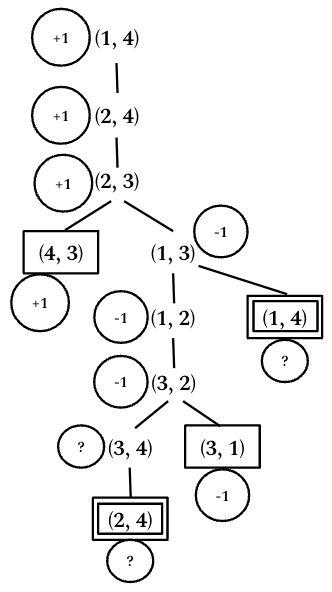
\includegraphics[scale=0.5]{472-PS4-Q1-B.png}

    % -------------------------------------------------------------------------------

    % ----------------------------------- 1c DONE -----------------------------------

    \item \textbf{(7 pts)} Explain why the standard minimax algorithm would fail on this game tree and briefly sketch how you might fix it, drawing on your answer to (b). Does your modified algorithm give optimal decisions for all games with loops?

    \color{blue}
        The minimax algorithm relies on recursion with a base case that terminates the recursion due to reaching a terminal node. In this game tree, we see loops created. Since minimax explores all possible actions, it will never end up terminating since it will always explore the action that leads to the loop over and over again. One way I would modify the algorithm is by implementing a dictionary (like a Hashmap) to detect if a state has already been reached (gives us a loop). If the state results in a loop, ignore that action and explore the others. This prevents loops and will help it eventually terminate, thus giving a functional minimax algorithm. My modified algorithm should give optmial decisions because, like I mentioned in part (b), the loop will never lead to a more optimal solution. The loop essentially "delays the inevitable", so ignoring the action that results in a loop will allow the algorithm to function with actions that progress the game.
    \color{black}

    % -------------------------------------------------------------------------------

    % ----------------------------------- 1d DONE -----------------------------------

    \item \textbf{(6 pts)} This 4-square game can be generalized to $n$ squares for any $n > 2$. Prove that $A$ wins if $n$ is even and loses if $n$ is odd.

    \color{blue}
        Basically, this game is a race to the other side. Therefore, the initial moves by both players need to be towards the middle. Otherwise, they are losing advantage by moving backwards and being further from their goal. So, in the case where $n$ is even, when they reach the middle, Player $A$ gets to jump Player $B$. The opposite happens when $n$ is odd. When the player jumps the other in this situation, the only way for the other player not to lose is to jump back over them (back towards their starting spot) since they would lose the "foot race" to the goal square. But, this makes them further from their goal and the only way for them to prevent their opponent from winning is to land back in their starting spot first. This blocks their opponent from moving to that spot. However, that player has to move backward, which then you can only move forward, and then they just jump over you and you win.\\

        This can happen with 6 squares. Both players must move towards the middle. They meet at $(3,4)$ and it is player $A$'s turn. They jump player $B$. If player $B$ tries to move forward to reach the goal, they are too far behind since player $A$ was already at the advantage of moving first, but then having a net of $+2$ squares for jumping player $B$. So, in a futile attempt to block player $A$, player $B$ decides to jump over them. This results in them being at $(5,6)$. Player $A$ only has one option, which is to move to square 4. This leaves player $B$ as only able to move to square $5$. Which, player $A$ simply jumps player $B$ to win.
    \color{black}

    % -------------------------------------------------------------------------------
    
    \end{enumerate}

% ----------------------------------------------------------------------------------

% ------------------------------------- 2 DONE -------------------------------------

\item \textbf{(14 pts)} (Exercise 5.9) This problem exercises the basic concepts of game playing, using tic-tac-toe (noughts and crosses) as an example. We define $X_n$ as the number of rows, columns, or diagonals with exactly $n$ $X$’s and no $O$’s. Similarly, $O_n$ is the number of rows, columns, or diagonals with just $n$ $O$’s. The utility function assigns +1 to any position with $X_3 = 1$ and $-1$ to any position with $O_3 = 1$. All other terminal positions have utility 0. For nonterminal positions, we  use a linear evaluation function defined as Eval($s$) $ = 3X_2(s) + X_1(s) - (3O_2(s) + O_1(s))$.

\begin{enumerate}[label=($\alph*$)]
    
    % ----------------------------------- 2a DONE -----------------------------------
    
    \item \textbf{(3 pts)} Approximately how many possible games of tic-tac-toe are there?

    \color{blue}
        $3^9 = 19683$ (since there are 9 spaces and each have 3 choices: $X$, $O$, or empty)
    \color{black}

    % -------------------------------------------------------------------------------

    % ----------------------------------- 2b DONE -----------------------------------

    \item \textbf{(4 pts)} Show the whole game tree starting from an empty board down to depth 2 (i.e., one $X$ and one $O$ on the board), taking symmetry into account.

    \color{blue}
        (Sorry for the uneven levels, couldn't fit them all in a row)
    \color{black}

    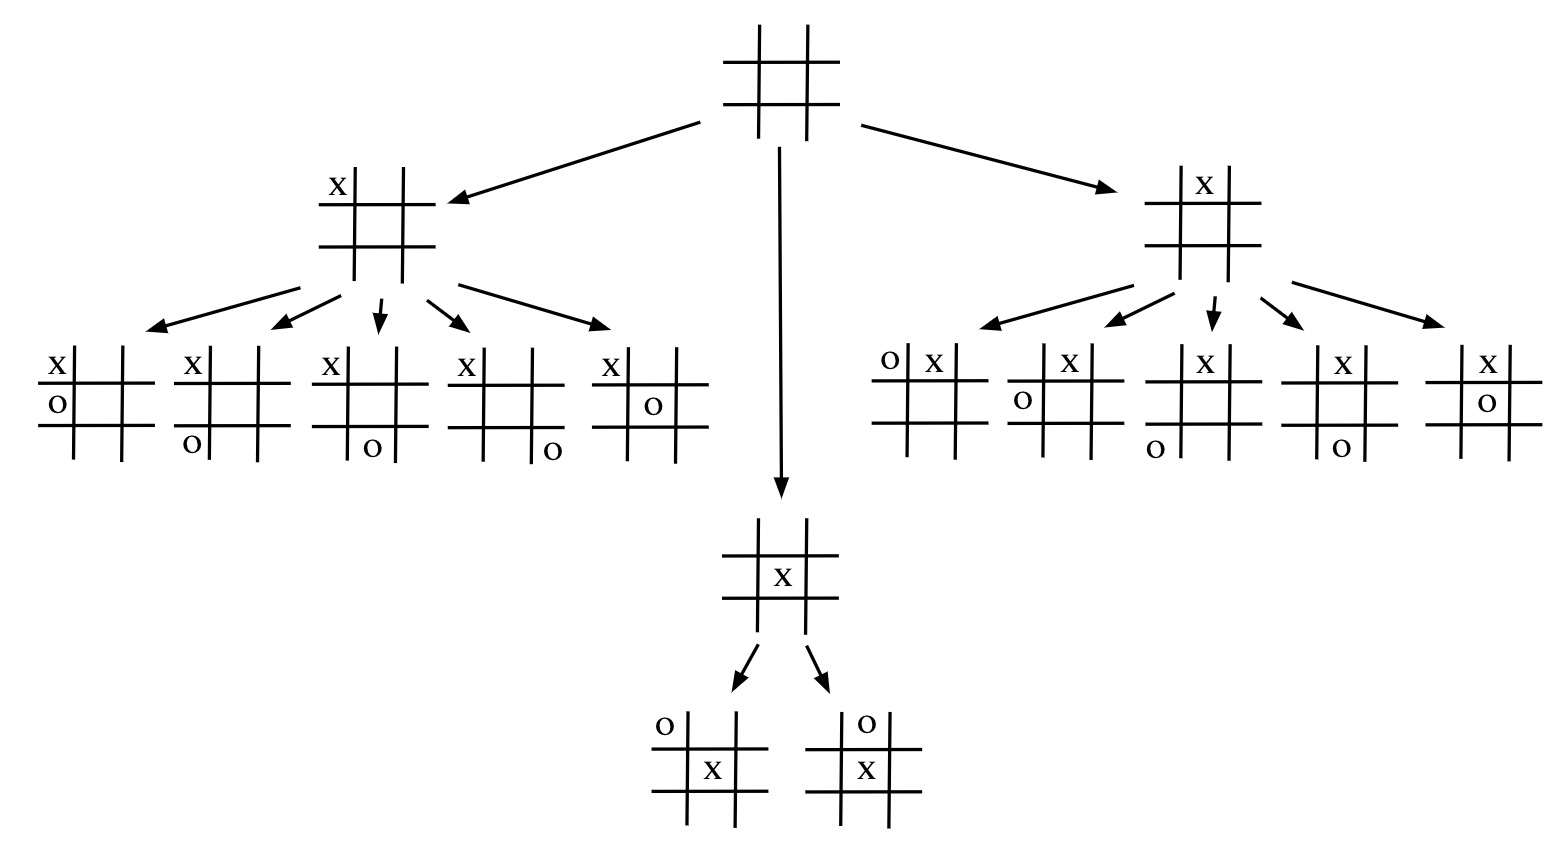
\includegraphics[scale=0.5]{472-PS4-Q2-B.png}

    % -------------------------------------------------------------------------------

    % ----------------------------------- 2c DONE -----------------------------------
    
    \item \textbf{(3 pts)} Mark on your tree the evaluations of all the positions at depth 2.

    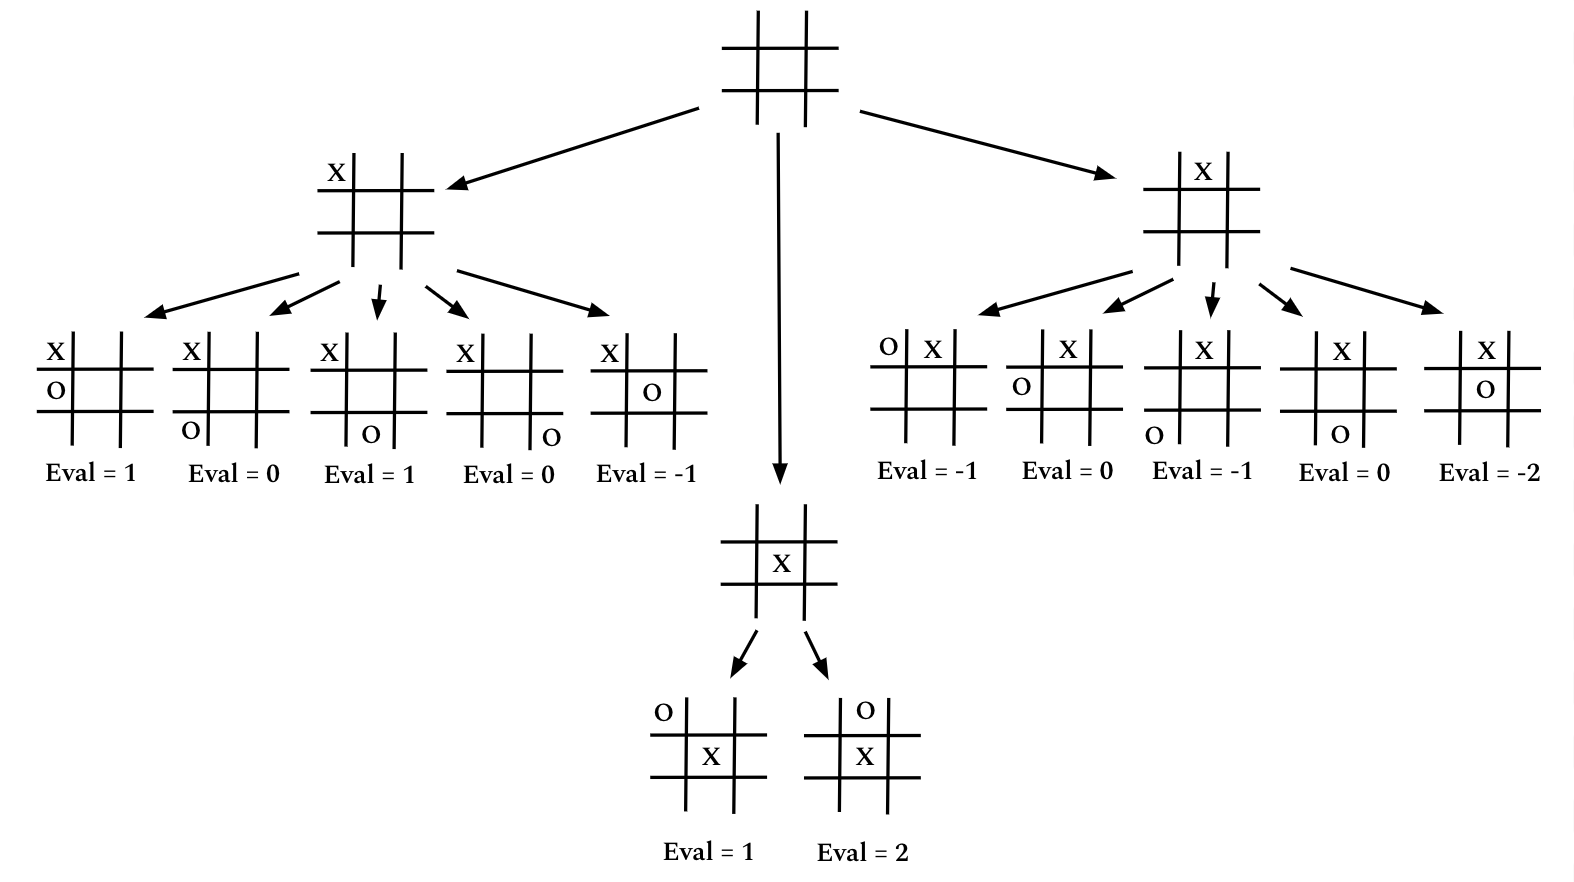
\includegraphics[scale=0.5]{472-PS4-Q2-C.png}

    % -------------------------------------------------------------------------------

    % ----------------------------------- 2d DONE -----------------------------------
    
    \item \textbf{(4 pts)} Using the minimax algorithm, mark on your tree the backed-up values for the positions at depths 1 and 0, and use those values to choose the best starting move.

    \color{blue}
        The best starting move is to put $X$ in the middle.
    \color{black}

    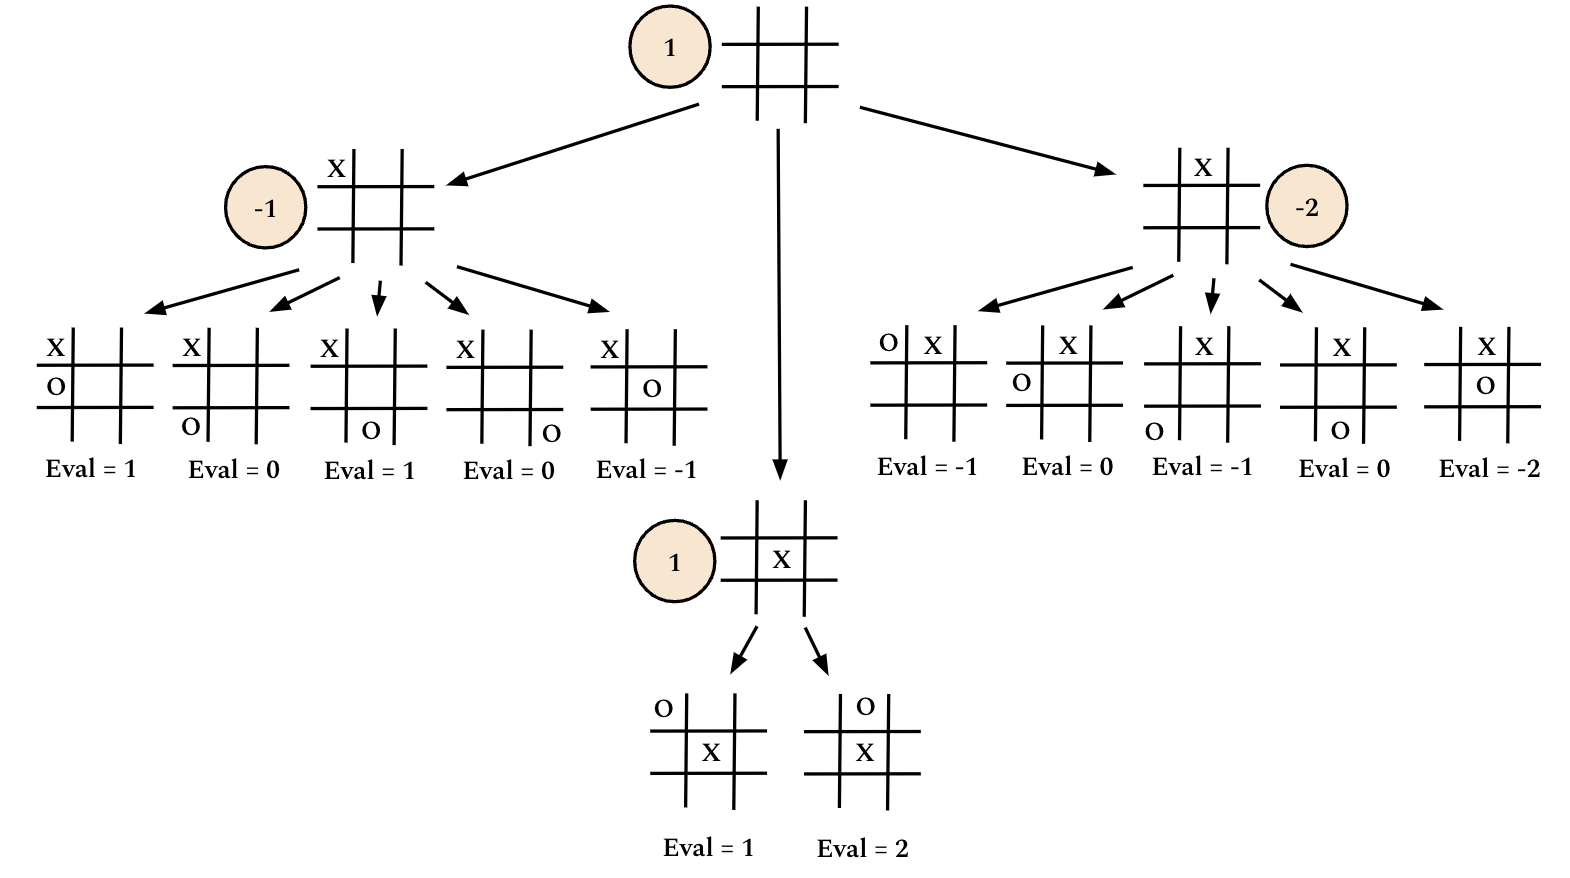
\includegraphics[scale=0.5]{472-PS4-Q2-D.png}

    % -------------------------------------------------------------------------------

    \end{enumerate}

% ----------------------------------------------------------------------------------

% ------------------------------------- 3 DONE -------------------------------------

\item \textbf{(18 pts)} You are given a minimax search tree as shown below. The tree has nine internal nodes $A, B, . . . , I$. Not all terminal states (leaves) are at the same depth. Execute the alpha-beta pruning algorithm (use the version from the 3rd edition of the textbook in the lecture notes on September 25).

\begin{center}
    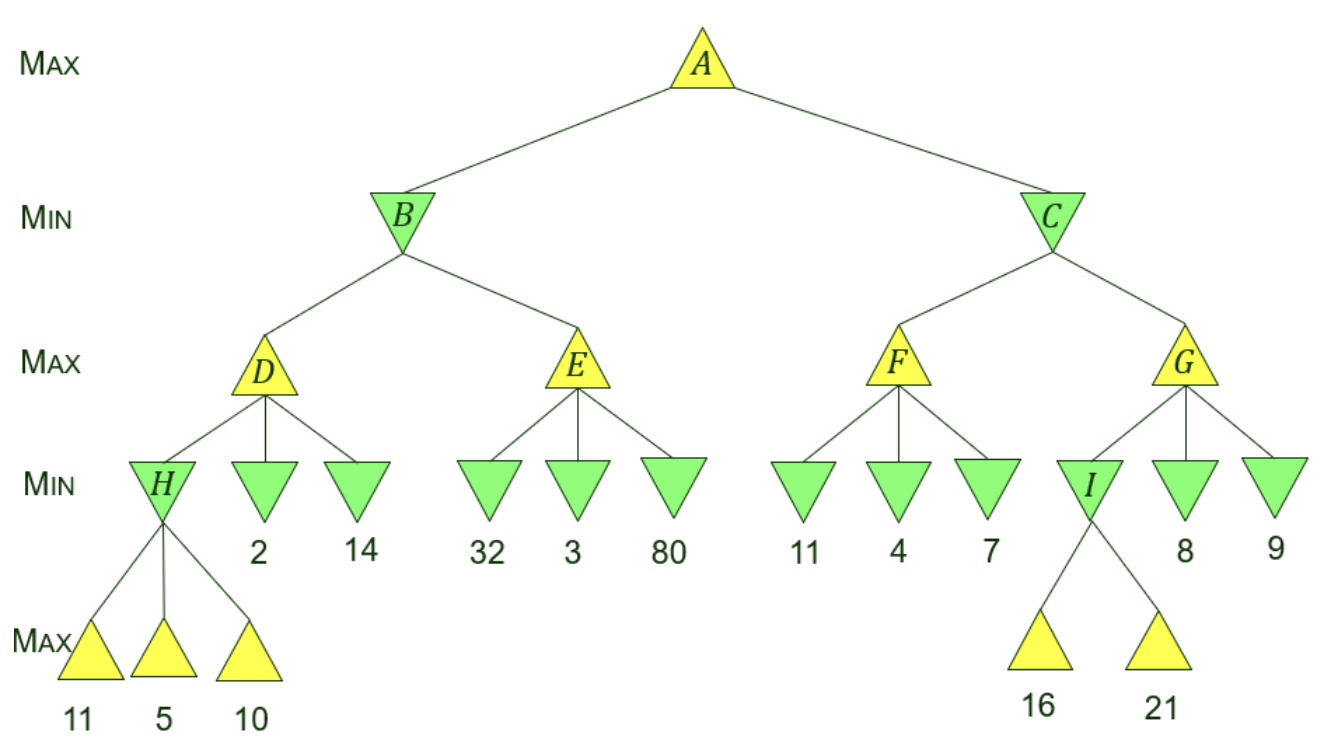
\includegraphics[scale=0.5]{472-PS4-Q3.png}
\end{center}

\begin{enumerate}[label=($\alph*$)]

    % ----------------------------------- 3a DONE -----------------------------------

    \item \textbf{(6 pts)} Mark all the subtrees (including leaves) that have been pruned. You may, for instance, simply put double slashes $\backslash\backslash$ or // across the edge entering the root of such a subtree from the above.

    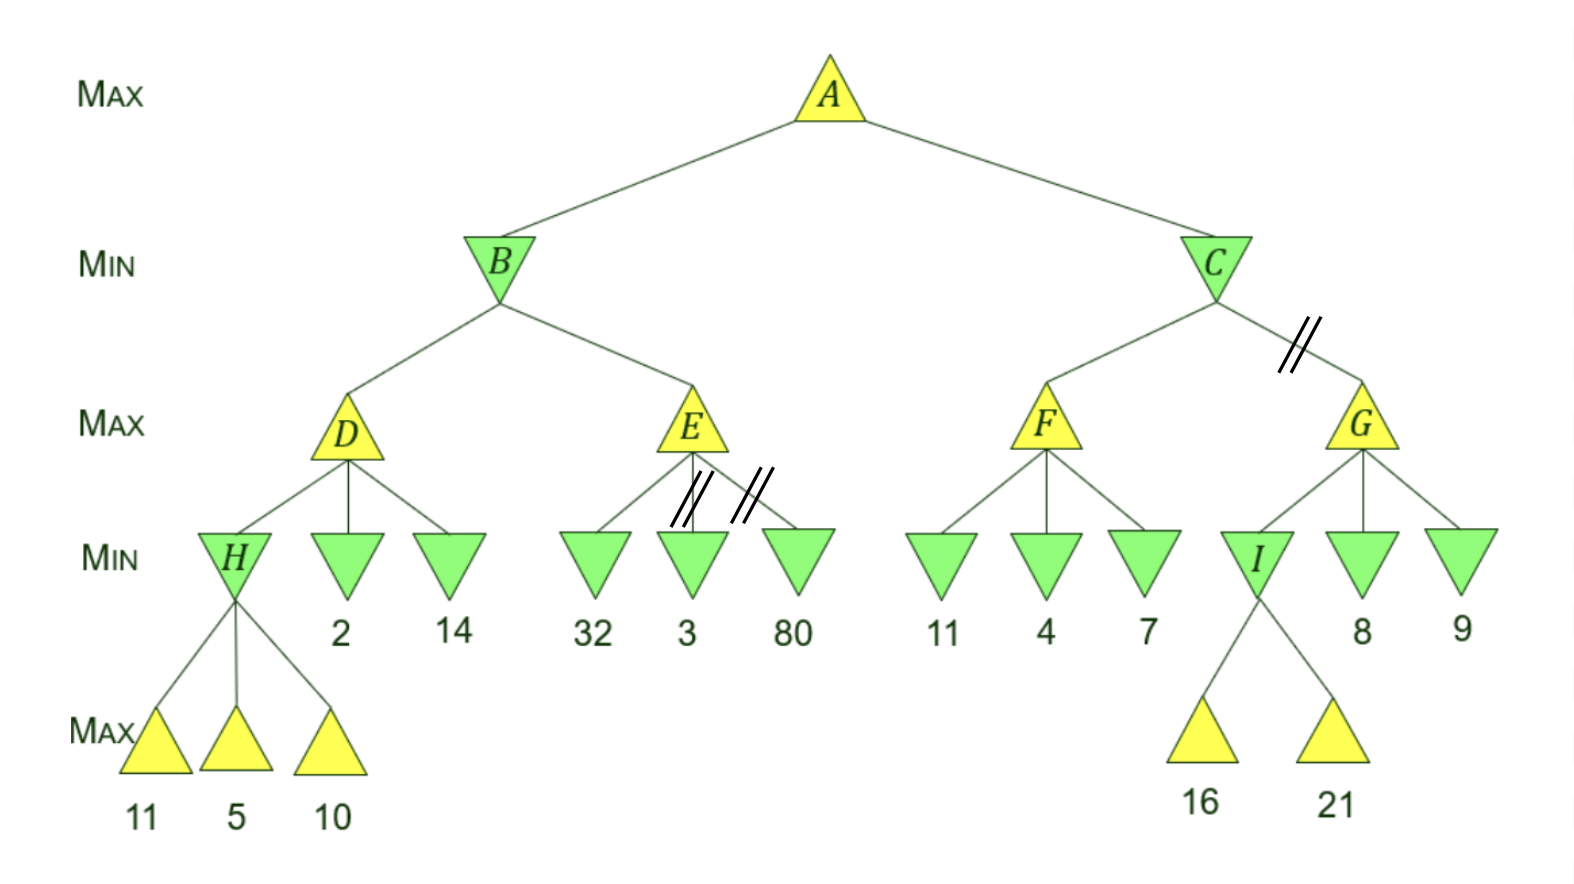
\includegraphics[scale=0.5]{472-PS4-Q3-A.png}

    % -------------------------------------------------------------------------------

    % ----------------------------------- 3b DONE -----------------------------------
    
    \item \textbf{(9 pts)} Next to each visited internal node, write down the two values $[\alpha, \beta]$ \textit{just before the return} from the call MAX-VALUE or MIN-VALUE invoked on the state represented by the node.

    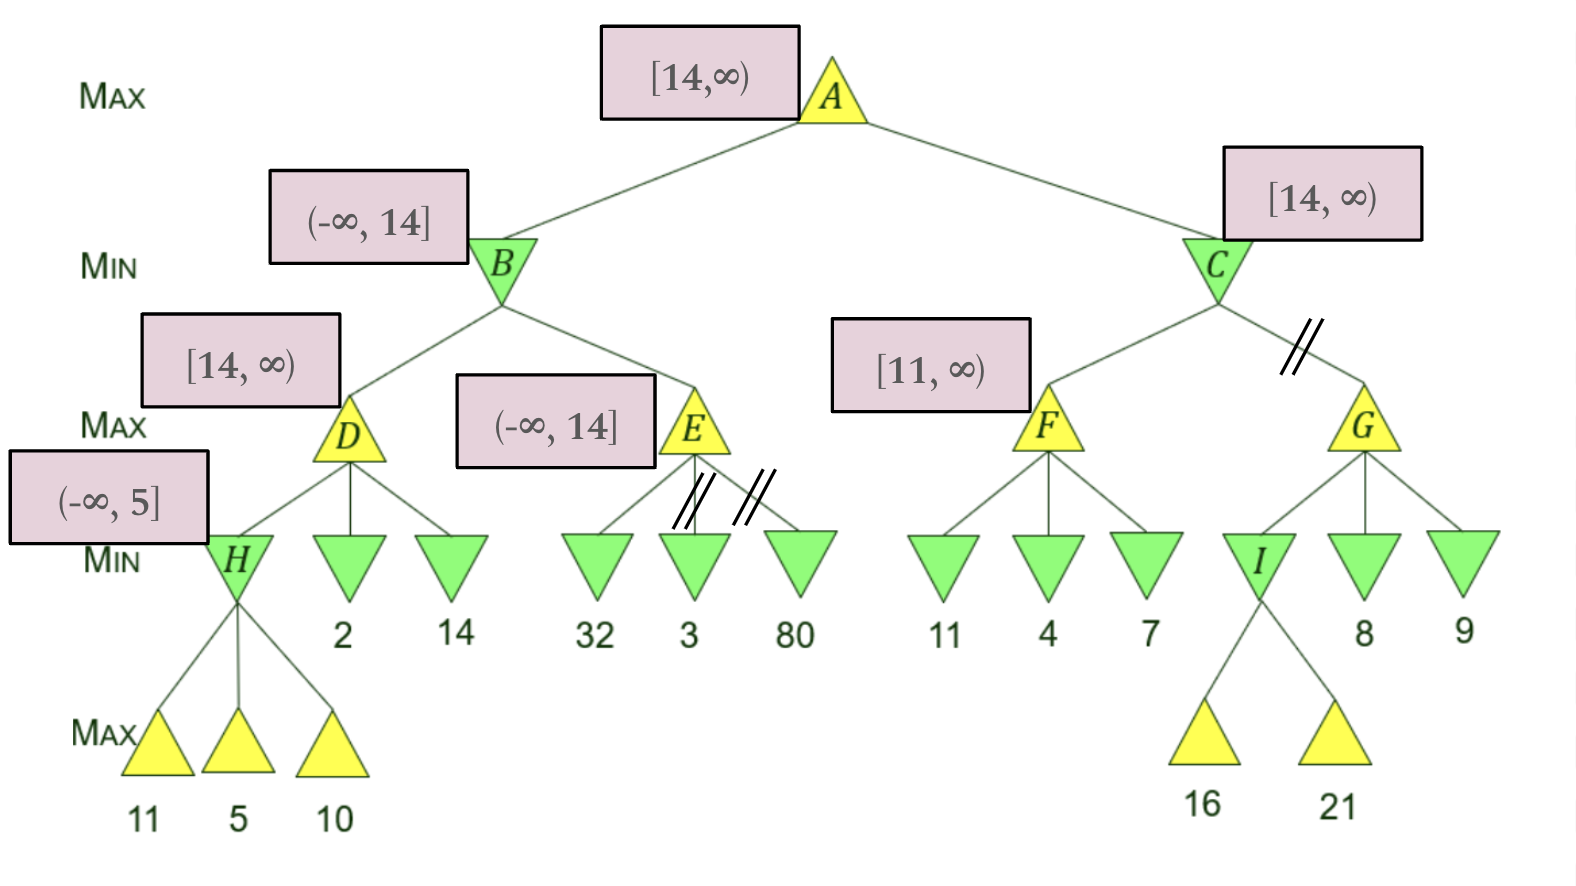
\includegraphics[scale=0.5]{472-PS4-Q3-B.png}

    % -------------------------------------------------------------------------------

    % ----------------------------------- 3c DONE -----------------------------------
    
    \item \textbf{(3 pts)} What is the final value for MAX at the root?

    \color{blue}
        The final value for MAX at the root is 14
    \color{black}

    % -------------------------------------------------------------------------------

    \end{enumerate}

% ----------------------------------------------------------------------------------

\end{enumerate}
\end{document}